\documentclass[conference]{IEEEtran}
%Template version as of 6/27/2024

\usepackage{cite}
\usepackage{amsmath,amssymb,amsfonts}
\usepackage{algorithmic}
\usepackage{graphicx}
\graphicspath{{images/}}
\usepackage{textcomp}
\usepackage{xcolor}
\def\BibTeX{{\rm B\kern-.05em{\sc i\kern-.025em b}\kern-.08em
    T\kern-.1667em\lower.7ex\hbox{E}\kern-.125emX}}
% \setlength{\parindent}{1em}
% \setlength{\parskip}{0.8em}
\begin{document}

\title{Neural Networks for Neural Tumors}

% old author block
% \author{
% \IEEEauthorblockN{\large Joe Vogel}
% \IEEEauthorblockA{\textit{UC Davis Computer Science} \\
% jvogel@ucdavis.edu}

% \and
% \IEEEauthorblockN{\large Nam Nguyen}
% \IEEEauthorblockA{\textit{UC Davis Computer Science} \\
% ncnn@ucdavis.edu}

% \and
% \IEEEauthorblockN{\large Jonathan Mo}
% \IEEEauthorblockA{\textit{UC Davis Computer Science} \\
% jtnmo@ucdavis.edu}

% \and
% \IEEEauthorblockN{\large Aryan Karnwal}
% \IEEEauthorblockA{\textit{UC Davis Computer Science} \\
% akarnwal@ucdavis.edu}

% \and
% \IEEEauthorblockN{\large Richard Ho}
% \IEEEauthorblockA{\textit{UC Davis Computer Science} \\
% rdho@ucdavis.edu}
% }

\author{
\centering
\begin{minipage}[t]{0.9\textwidth}
  \centering
  \begin{tabular}{ccc}
    Joe Vogel & Nam Nguyen & Jonathan Mo \\
    \textit{UC Davis Computer Science} & \textit{UC Davis Computer Science} & \textit{UC Davis Computer Science} \\
    jvogel@ucdavis.edu & ncnn@ucdavis.edu & jtnmo@ucdavis.edu \\
    \vspace{0.6em}
  \end{tabular}
  \begin{tabular}{cc}
    Aryan Karnwal & Richard Ho \\
    \textit{UC Davis Computer Science} & \textit{UC Davis Computer Science} \\
    akarnwal@ucdavis.edu & rdho@ucdavis.edu \\
  \end{tabular}
\end{minipage}
}

\maketitle

\begin{abstract}
This report documents the process of creating a machine learning model that classifies brain tumors given MRI brain scan imagery. This project saw the creation of three successful models using the following algorithms: Convolutional Neural Network, Support Vector Machine, and Random Forest. 
\end{abstract}

\begin{IEEEkeywords}
Brain tumor classification, Convolutional Neural Network (CNN), MRI brain imagery, Random Forest (RF), Support Vector Machine (SVM). 
\end{IEEEkeywords}

\large 
\section{\large Introduction (Front page)}
As a team of five young computer science students with no prior machine learning experience, we ambitously decided to tackle the real world challenge of brain tumor classification for our \textit{ECS 171 - Machine Learning} final project at UC Davis. Through hours and hours of research and trial and error, we learned a lot, and we have a lot to share. 

We hope this report serves not only as an informative summary of our findings, but also as motivation for your own projects. We faced many challenges during this project, but in the end created something we are all very proud of, despite our lack of experience.

\subsection{\large Motivation}

Brain tumors make up for... reference 9% TODO

Hundreds of thousands of MRI brain scans are performed every day. With the scans being so intricate, it can sometimes be hard for even a trained professional to determine whether or not a patient has a brain tumor, and even harder to tell which kind. 

Having a tool that could detect and identify tumors within seconds, and with high accuracy, would save a lot of time and money. Not to mention the impact it would have on developing nations who might not have as many specially trained doctors that can readily perform MRI analysis. With lives on the line, early detection is absolutely key to diagnosing and treating these tumors.

\subsection{\large Approach}
A classification machine learning model is a great approach to this problem. Using a convolutional neural network and an image dataset, we can train a model to accuractely classify brain tumors. With its complex neural structure, such a model can detect nuances and patterns in the scans that are otherwise hard to spot. This project used a dataset that focused on three brain tumor types: glioma, meningioma, pituitary. Along with the three tumor types, the model should also be able to classify scans as "no tumor". The aim for this model was to predict tumor classes with over 95\% accuracy.

\section{\large Literature Review (Complete)}

\subsection{\large Brain Tumor Classification in MRI Image Using Convolutional Neural Network$^{1}$}

In this article from 2021, authors Khan et al. examine convolutional neural network models for brain tumor classification, reporting classification accuracies ranging from 80\% to 98\%. The authors highlight two primary challenges in training such models: (1) the scarcity of accurately labeled data, which increases training complexity and cost, and (2) inconsistency in image dimensions, given that CNNs require fixed-size input. Their dataset is partitioned into training, validation, and testing sets, serving model training, hyperparameter tuning, and final evaluation, respectively. Image pre-processing is performed using Canny Edge Detection, an open-source computer vision technique. To address the limited dataset size, the authors employ data augmentation methods such as flipping, rotation, and brightness adjustments to enhance variability. The model utilizes the ReLU activation function and stochastic gradient descent for optimization.

Given our limited computational resources, we plan to utilize a pre-trained model. The eight-layer architecture discussed in the paper provides a useful baseline. The pre-processing techniques mentioned are also great starting points for us, and let us know what we should look out for. Furthermore, we intend to implement data augmentation techniques to improve generalization on our small dataset. The use of ReLU and stochastic gradient descent aligns well with our current understanding, and we aim to assess their impact on our model's performance.

\subsection{\large A Deep CNN Based Multi-Class Classification of Alzheimer's Disease Using MRI$^{2}$}

In this article, Farooq, Anwar, Awais, and Rehman demonstrate their implementation of a four-way Alzheimer's disease classifier. Considering their model also takes MRI imagery as input and has four class target labels, we can learn a lot from their experiments. The authors began their model development with data preprocessing and a technique known as skull stripping, which is the process of removing non-brain tissues like the skull or fat from MRI imagery. We could implement skull stripping in our model to improve the signal-to-noise ratio and reduce input complexity, which could help against overfitting. 

Additionally, the article mentions the utilization of data augmentation to increase the data set; they simply flipped the images along the horizontal axis, which is valid due to the left and right symmetry of the brain. This method increased their dataset from 355 MRI volumes to 38024 images. We can implement the same method in our project because increasing the sample size can combat overfitting, making our model more accurate.

\subsection{\large Brain Tumor Classification Using Convolutional Neural Networks$^{3}$}

In this publication, authors Seetha and Raja demonstrate the effectiveness of convolutional neural networks for brain tumor classification. Their proposed CNN-based classification approach achieves an impressive 97.5\% accuracy rate while maintaining low computational complexity compared to other methods. Seeing such a high accuracy be achieved is both inspiring and motivating for us. Considering their model also predicts four tumor types, their high accuracy rate sets a benchmark we should aspire to, and their focus on computational efficiency aligns with our resource constraints. 

The authors implemented a deeper architecture design using small kernels, with neuron weights intentionally kept small to optimize performance. Their experimental results demonstrated that their CNN model outperformed other state-of-the-art methods in both accuracy and efficiency. Like our approach, they used a dataset containing various brain MRI scans and faced similar challenges with image preprocessing. Their optimization of kernel size and weight parameters offers valuable insights for our model development. Given that our initial prototype showed signs of overfitting (93\% training accuracy with 42\% testing accuracy), we should consider implementing some of the suggested architectural decisions regarding smaller kernels and weight optimizations, while continuing with our planned transfer learning approach to improve generalization.


\section{\large Dataset Description (1 page)}

The dataset used for this project comes from a group of brilliant students at Savitribai Phule Pune University in India. It is an open source dataset that can be found for free on Kaggle\textsuperscript{4}. It is a well respected and reviewed dataset. The dataset consists of 3264 labeled MRI scan images. The images are divided into four categories. There are three different tumor types, and one set of “no tumor” scans. Because each image in our dataset is already classified, our model's training is considered supervised, as opposed to unsupervised, where each training image would not have an associated classification. An unsupervised model would require a much different approach, most likely using different algorithms.

\subsection{\large Preprocessing}

Due to the non-numerical nature of image datasets, our input features come in a different form than they normally would with a numerical dataset. Instead of having numerically represented features such as 'age', 'blood pressure', and so on, our dataset only has images. Technically, each image is a set of numbers (pixel intensities), but the idea remains. We don't really have a standard feature selection process, or get to choose which features to train our model on. Instead, things like image preprocessing and model hyperparameters are key to training an accurate model.

Preprocessing steps might include things like image resizing, cropping, normalization, and data augmentation (rotating, flipping, zooming, etc.). We can even consider techniques like 'skull stripping', used to isolate only the brain, since we do not care about anything else in the scan.

\section{\large EDA (1 page)}

% EXAMPLE image in a column
% \begin{figure}[!ht]
%     \centering
%     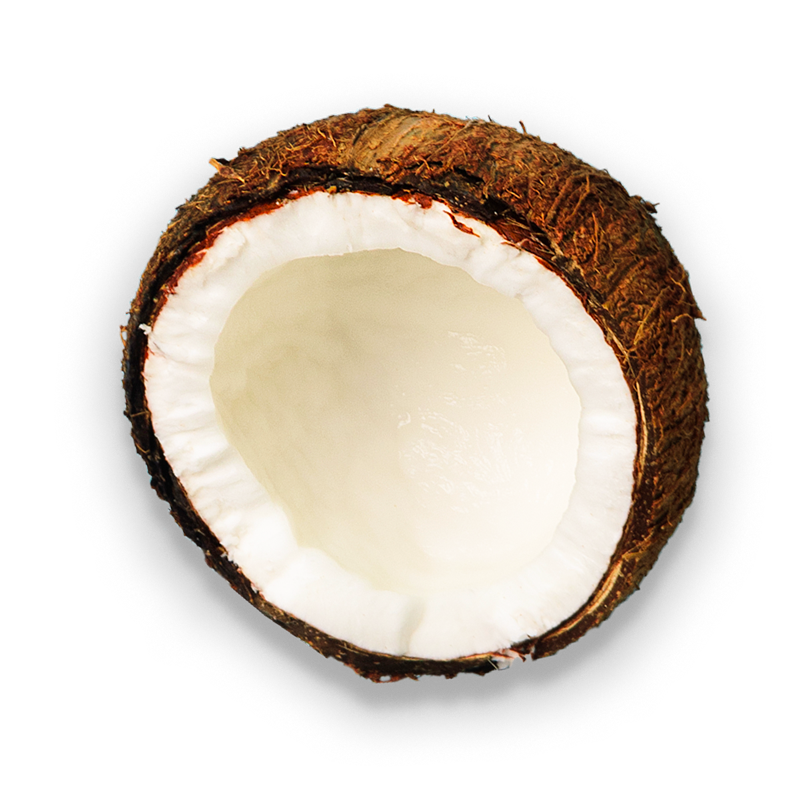
\includegraphics[width=2in]{coconut.png}
%     \caption{this is a coconut}
%     \label{test image coconut}
% \end{figure}

% EXAMPLE image across two columns
% \begin{figure*}[!ht]
%     \centering
%     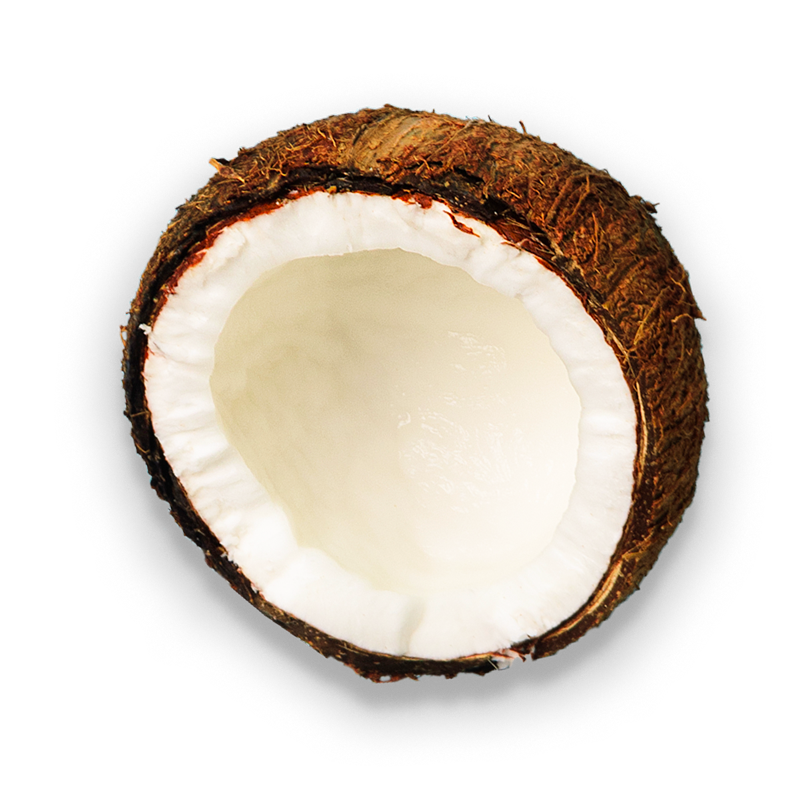
\includegraphics[width=3in]{coconut.png}
%     \caption{this is a coconut}
%     \label{coconut}
% \end{figure*}

% These two won't stay in the same row
% \begin{figure*}[!ht]
%     \centering
%     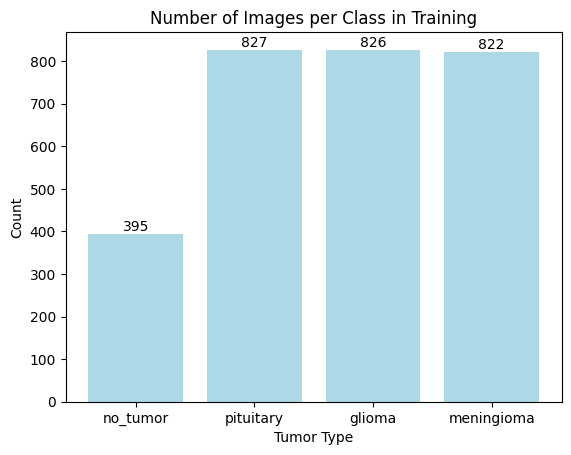
\includegraphics[width=1in]{ImagesPerClassTraining.png}
%     \caption{\large Images in the training dataset}
%     \label{Number of images per class in the training dataset}
% \end{figure*}

% \begin{figure*}[!ht]
%     \centering
%     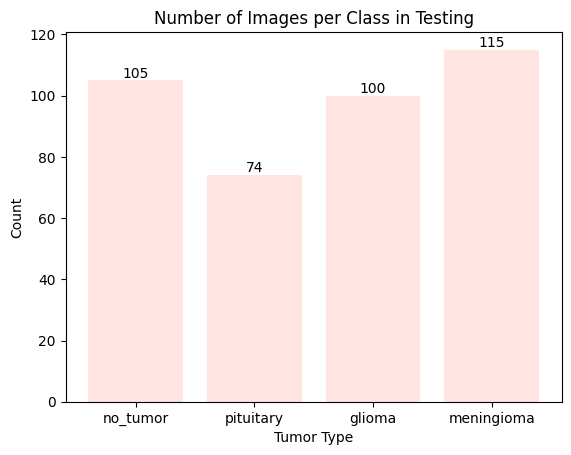
\includegraphics[width=1in]{ImagesPerClassTesting.png}
%     \caption{\large Images in the testing dataset}
%     \label{Number of images per class in the testing dataset}
% \end{figure*}

% Both figures in one row
% TODO: Move these to be under EDA in the right spots
\begin{figure*}[!ht]
    \centering
    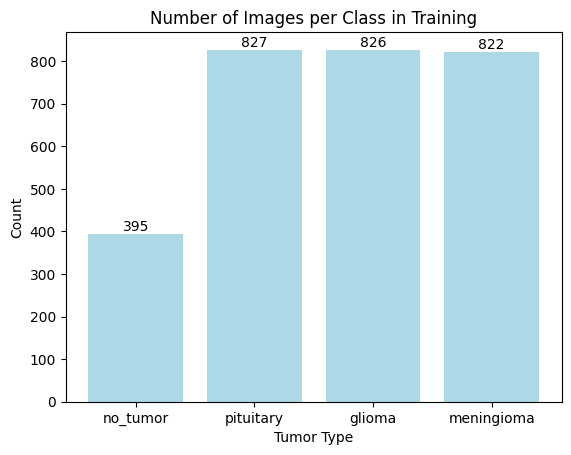
\includegraphics[width=0.49\textwidth]{ImagesPerClassTraining.png}
    \hfill
    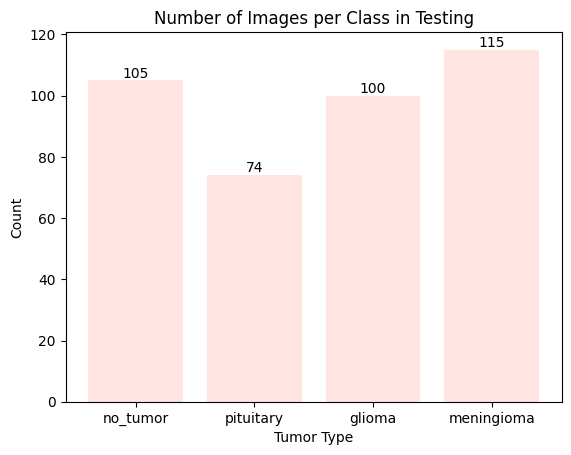
\includegraphics[width=0.49\textwidth]{ImagesPerClassTesting.png}
    \caption{\large The dataset has a consistent number of training images across classes, except for "no tumor". This should not be an issue because "no tumor" imagery has much less variance. For testing, the distribution of images is more varied, but this does not affect model performance, since the model is not trained on this data at all.}
    \label{fig:images-per-class}
\end{figure*}

As we can see in Figure 1 (left), there is an even distribution of images among each class (~825), except for the no tumor class (395). This is because the images without tumors have much less variance. We expect it to be much easier for the model to detect "no tumor", and we do not think the lower number of images in the "no tumor" class will have a negative effect on the model's ability to classify images as such. However, if we do see poor results in that classification specifically, we can try changing all classes to train on 395 images, to see if that helps with the class-specific overfitting. Additionally we could also focus our data augmentation on the "no tumor" class, bringing its number of images up to the others.

In our test dataset seen in Figure 1 (right), we have a much more uneven distribution among each class. This of course won't affect our model's ability, since it is not being trained on this data, but some results could be skewed considering the relatively low number of pituitary images. It could be useful to test against more pituitary imagery to ensure the model can handle all variations of scans. We could again perform data augmentation and create more pituitary data by rotating, zooming, and flipping our existing images. Testing against more data could give us more confidence in our model, if scores remain high.

\begin{figure*}[!ht]
    \centering
    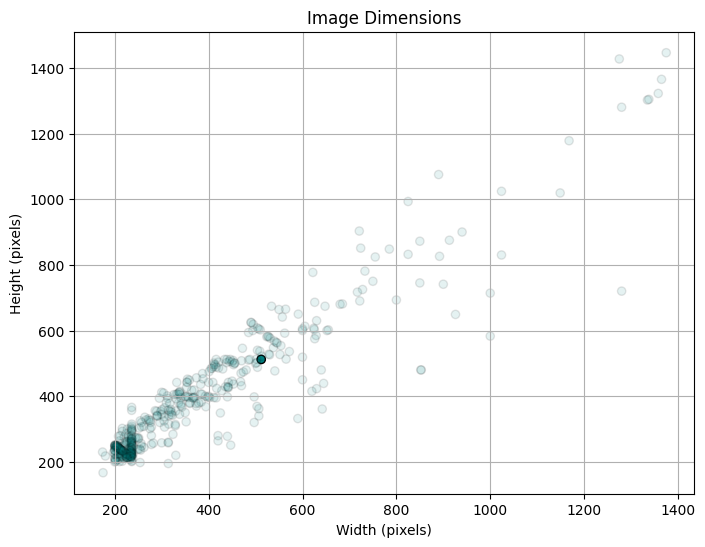
\includegraphics[width=4in]{ImageDimensions.png}
    \caption{\large It is clear to see the images in the dataset are of many varying dimensions. We do see higher densities around the 200x200 and 500x500 dimensions, though. Regardless, such variation means image preprocessing and resizing is necessary before training.}
    \label{Dimensions of images in the dataset}
\end{figure*}

We can see in Figure 2 that our dataset is comprised of images of many varying sizes. There seems to be a concentration around the 200x200 and 500x500 sizes. With this information, we know we will have to perform some image pre-processing to convert all images into the same size so the model has consistent input. We will provide our CNN with the conventional 224x244 image dimensions.

\section{\large Methodology (1-2 pages)}

\subsection{\large Feature Selection}
As mentioned in our dataset description, we don't have labels for our input features like a numerical dataset would have. We only have our images, which are technically each a set of pixel intensity values, but it means we can't select certain features to train our dataset on. Instead, we can perform some image preprocessing and hyperparameter tuning to increase our model's accuracy.

Looking at Figure 3 again, we see all of our images have different dimensions. As a preprocessing step, we will resize them all to be 224x224 pixels, so that our model has consistent input.  The resizing step is not as simple as it sounds though, we must be careful because shrinking or enlarging our images can create unwanted noise in our data. After imagine resizing, we then normalize each pixel's value from its 3-channel RGB form.

Our training dataset consists of 2870 MRI scans. If we want to give our model more images to train on, we can perform data augmentation like mentioned previously. We can rotate, flip, and zoom our images to create 'artificial' data that will hopefully prevent overfitting and allow for our model to capture underlying patterns better. We also hope this will allow for our model to predict against a larger variety of testing data (i.e. rotated images). 

The hyperparameters of our model are crucial to achieving a good fit. In our first iteration of the model, some of the hyperparameters we chose were as follows:
%TODO --- fix table
- Image size: 256x256 pixels		- Batch size: 32		- Epochs: 30	
- Loss:  Categorical Cross Entropy 	- Metrics: Accuracy		- Dropout Rate: 0.25 and 0.50
We plan on fine tuning these parameters with techniques like grid search as we continue to optimize our model. 

\subsection{\large Early Model Development}

Our first early prototype was a CNN model with 4 convolutional blocks, followed by fully connected layers using the Keras Sequential API. We trained the model over 30 epochs, with each epoch giving us higher accuracy on the training data, peaking at 93\% after the last epoch. However, when performing predictions on our testing data, the model saw a big dip in performance. With an average accuracy of 42\%, our model was heavily overfitting on the training data.

% @Nam is this true? k-fold CV etc.?
To improve upon our first model, we applied k-fold cross validation and tuned hyperparameters such as dropout rate, number of layers/neurons, etc. We implemented grid search to tune our hyperparameters. We also planned to use transfer learning to reduce the number of learned parameters and implicitly filter irrelevant features, which can greatly reduce overfitting risks. Going forward, we'd use PyTorch, which gave us more flexibility in controlling forward pass, backpropagation, and optimization, allowing us to develop a better CNN model.

\section{\large Experimental Results (2 pages)}
Talk about trying three different models, different pretrained models like ResNet, (the other one you tried first Nam I forgot what it was)

Talk about fine-tuning, grid search for hyperparameter fine-tuning, etc.

Nam, Elaborate on this: "Alright guys, I finally figured out the problem. I've been using different pre-trained models but keep ending up with a lot of false negatives for the class glioma. I reviewed another notebook using the same dataset. Comparing it with our reference notebook, I notice that they both initially combined the training and testing folders, shuffled and split again. On the other hand, I'd been using the dataset as it is split on Kaggle. I believe there must be significant patterns in the testing folders on Kaggle that are not present in the training ones, especially the glioma-tumor class. So, merging them together and splitting again is the optimal solution here. Btw, I also decided to use Keras Function API instead of Sequential API (still same network architecture) and it turned out to be slightly better. I run the model several times and the accuracy is averagely around 92\% to 95\%"

\section{\large Evaluation (1-2 pages)}
In this project, three machine learning models—Convolutional Neural Networks (CNN), Support Vector Machines (SVM), and Random Forests (RF)—were trained and evaluated. In this section, the performance of these models are assessed using standard classification metrics, including accuracy, precision, recall, and F1 score. The dataset utilized for this evaluation consists of four classes: glioma, meningioma, pituitary tumor, and no tumor.

The CNN model demonstrated the highest overall accuracy at 96.68\%, followed closely by SVM at 95.66\%, and RF at 94.90\%. Macro and weighted F1-scores mirrored this trend, with CNN achieving 0.97, SVM 0.96, and RF 0.95 in both averages. These scores indicate that CNN not only achieves better overall classification performance but also maintains consistency across classes in terms of precision and recall.

Diving into per-class specifics, we observe that for the label "glioma", CNN exhibited the highest precision (0.98) and recall (0.93), indicating strong identification capability with few false positives and a relatively low false negative rate. SVM matched CNN in precision (0.98) but had a lower recall (0.91), while RF also had a precision (0.98) but the lowest recall score at 0.89. This suggests that both SVM and RF are more likely to miss "glioma" cases compared to CNN while matching its precision.

In the case of "meningioma", while CNN had the best precision (0.93), SVM and RF had equal or superior recall (0.97 and 0.98 respectively) compared to CNN (0.97). SVM and RF had reduced precision (0.89 and 0.87) which is a notable difference from CNN's aforementioned score. This pattern indicates that SVM and RF are more sensitive in detecting "meningioma" but may yield more false positives than CNN.

In classifying "no tumor", RF achieved perfect precision (1.00), which means that every time RF predicted "no tumor", the model was correct. However, its recall (0.93) was the lowest among the three, pointing to a higher rate of false negatives. CNN balanced both precision (0.97) and recall (0.98) well, outperforming both alternatives in overall reliability for this class.

For the label 'pituitary', all three models performed strongly, with CNN leading both in precision and recall (0.99 each). SVM and RF followed closely with both metrics at 0.98 and 0.97-0.98, respectively, indicating that all models are highly effective in classifying "pituitary" tumors.

\section{\large Conclusion (1/2 page)}
The above evaluation highlights CNN's strength in handling complex, high-dimensional image data, likely due to its hierarchical feature extraction capability. Its superior balance in both precision and recall in all tumor types supports its suitability for real-world clinical deployment, where false positives and false negatives carry significant risk.

SVM performed comparably well, especially in the detection of meningioma and pituitary tumors, and may offer a lighter alternative in environments with limited computational resources. However, it showed reduced precision in some classes, which made it slightly less robust overall.

RF, while achieving remarkable precision, particularly for the "no tumor" class, exhibited reduced recall across multiple classes. This suggests a tendency to make fewer false positives, at the expense of missing actual tumor cases, which is a very serious and life-threatening issue in medical diagnostics.

\section{\large Our Team (1 page)}
The link to our GitHub\textsuperscript{8} repository for this project can be found in the references of this report.

project roadmap? Reference the first one pager outline assignment we did on google doc
%TODO --- roadmap?
\subsection{\large Demonstration}
include youtube video of our demo

\subsection{\large Roles and Contributions}

Joe: As the team leader, Joe has taken charge of organizing meetings, assigning tasks, and the general oversight over the project. In the coming weeks, Joe will be focusing on Exploratory Data Analysis, Literature Review, and Model Optimization. 

Nam: Nam took charge of making the first prototype of our model. Having this model as a starting and reference point is absolutely crucial in the development of subsequent models. In the next few weeks, Nam will be researching different frameworks and libraries to develop other CNN models to see which best fit our dataset.

Jonathan: Jonathan took charge of literature review and researched techniques that can be implemented to the model. In the next few weeks, Jonathan will be focusing on writing the proposed methodology for the final report.

Richard: Richard contributed to the project by evaluating the performance of the three machine learning model using evaluation metrics such as accuracy, F1 score, precision, and recall. Based on these analyses, he provided the rationale for selecting the CNN model as the final model due to its superior performance relative to the alternatives. Additionally, he conducted a comprehensive literature review to summarize key developments in the field, which served as a foundational reference for the project. His contributions also included performing exploratory data analysis (EDA) and preparing the dataset for modeling through appropriate data preprocessing techniques.

Aryan: Aryan completed a literature review and analyzed research papers to identify techniques we can use to address the models overfitting. In the next few weeks Aryan will continue working to improve the models accuracy while also working on documentation and reports. 

\begin{thebibliography}{00}

\bibitem{Khan2021}
H. A. Khan, W. Jue, M. Mushtaq, and M. U. Mushtaq, “Brain tumor classification in MRI image using convolutional neural network,” *Math. Biosci. Eng.*, 2021. 

\bibitem{Farooq2017}
A. Farooq, S. Anwar, M. Awais, and S. Rehman, “A deep CNN based multi-class classification of Alzheimer's disease using MRI,” in *Proc. IEEE Int. Conf. Imaging Syst. Tech. (IST)*, 2017, pp. 1-6. 

\bibitem{Seetha2018}
J. Seetha and S. S. Raja, “Brain tumor classification using convolutional neural networks,” *Biomed. Pharmacol. J.*, vol. 11, no. 3, p. 1457, 2018.

\bibitem{Sartaj2020}
Sartaj. “Brain Tumor Classification (MRI).” Kaggle, 24 May 2020, www.kaggle.com/datasets/sartajbhuvaji/brain-tumor-classification-mri. 

\bibitem{Kumar2014}
R. S. Kumar and M. Karnan, “Review of MRI image classification techniques,” *Int. J. Res. Stud. Comput. Sci. Eng.*, vol. 1, no. 1, pp. 21-28, 2014. 

\bibitem{Hasan2019}
A. M. Hasan, H. A. Jalab, F. Meziane, H. Kahtan, and A. S. Al-Ahmad, “Combining deep and handcrafted image features for MRI brain scan classification,” *IEEE Access*, vol. 7, pp. 79959-79967, 2019. 

\bibitem{Meier2020}
R. Meier, A. P. de Mortanges, R. Wiest, and U. Knecht, “Exploratory analysis of qualitative MR imaging features for the differentiation of glioblastoma and brain metastases,” *Front. Oncol.*, vol. 10, p. 581037, 2020.

\bibitem{Vogel2025}
J. Vogel, N. Nguyen, J. Mo, A. Karnwal, R. Ho, "Neural Networks for Neural Tumors". GitHub. https://github.com/Coco501/Neural-Networks-
for-Neural-Tumors

\bibitem{NBTS2022}
Brain tumor facts. National Brain Tumor Society. (2024, February 20). https://braintumor.org/brain-tumors/about-brain-tumors/brain-tumor-facts/ 

\end{thebibliography}


\end{document}